\documentclass[9pt,twocolumn,twoside]{styles/osajnl}
\usepackage{fancyvrb}
\journal{i524} 

\title{Couchbase Server: A Usable Overview}

\author[1]{Matthew Lawson}

\affil[1]{School of Informatics and Computing, Bloomington, IN 47408, U.S.A.}

\affil[*]{Corresponding authors: laszewski@gmail.com}

\dates{Paper1, \today}

\ociscodes{Couchbbase, Memcache, CouchDB, Cloud, I524}

% replace this with your url in github/gitlab
\doi{\url{https://github.com/eunosm3/classes/blob/master/docs/source/format/report/report.pdf}}


\begin{abstract}
Couchbase, Inc. develops Couchbase Server (CBS), an open-source, document-oriented, NoSQL database. Couchbase targets situations requiring high availability and high throughput of large amounts of data, i.e., big data.  CBS integrates Couchstore, Memcache and ForestDB, as well as a host of maintenance, administration and querying tools, in order to attempt to meet its promises to its users.  Corporate Couchbase users include General Electric (GE), LinkedIn Corp. and American Airlines, among others..
\newline
\end{abstract}

\setboolean{displaycopyright}{true}

\begin{document}

\maketitle

\section{Introduction}

Couchbase, Inc. offers Couchbase Server (CBS) to the marketplace as its entry in the NoSQL, \textit{big data} database field.  Salient features include a) an integrated cache tier which is essential to the product's operation; b) persistent storage in JSON document format, i.e. document-based storage, or simple key-value pairs; c) relatively uncomplicated scalability across clusters of commodity servers; d) sub-millisecond response times; e) a SQL-like query language; and, f) built-in cluster replication, failover and disaster recovery features.  In addition, Coucbhase markets a mobile product, Couchbase Mobile, which uses a Couchbase-designed syncing system to extend CBS to mobile devices and offline use cases.

\begin{figure*}[htbp]
\centering
\fbox{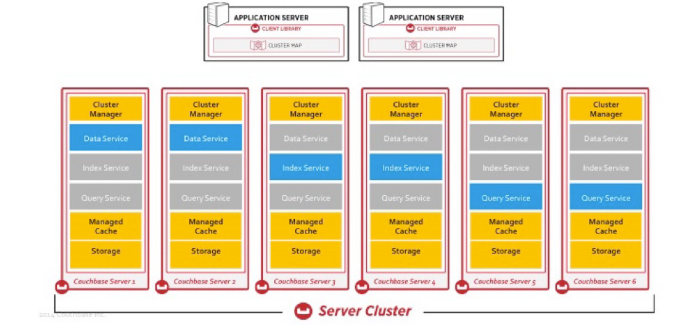
\includegraphics[width=\linewidth]{images/multiDimScaling}}
\caption{Multidimensional Scaling with Couchbase \cite{www-components-cbsinc}}
\label{fig:multidim scaling}
\end{figure*}

\section{Architecture} 

A Couchbase Server (CBS) system consists of at
least one cluster of interconnected servers running a copy of CBS. By
default, the CBS system's computers, referred to as nodes, work together in a master-master setup, which Couchbase calls a peer-to-peer topology \cite{www-components-cbsinc}.  In a master-master distributed cluster, the nodes co-exist in flat hierarchy, i.e., no node acts as the central authority.  Despite the egalitarian nature of the cluster, the nodes still need to coordinate activities.  Therefore, the nodes \textit{elect} a node to coordinate cluster functions. If the node fails or is removed from the cluster, the remaining  nodes elect a new \textit{orchestrator}.

In addition, the database administrator can override the default peer-to-peer topology by taking advantage of CBS' \textit{multi-dimensional scaling}.  This functionality allows the administrator to customize nodes to perform tasks for which the node is best suited, e.g., memory-intensive processes or I/O-intensive processes, etc.

A complete CBS system physically consists of a) one or more server clusters running the couchbase daemon; b) high-speed connections between the servers and between the clusters; and, c) client computer applications utilizing memcached-compatible software development kits, also known as \textit{devkits} or \textit{SDKs}.
\textbf{RESPONSE: I am not sure how to comply because this paragraph represents a portion of the mosaic of knowledge I now possess regarding CBS.  That is, it is an original thought.}.  

The main components of a Couchbase Server node consist of the following: a) the cluster manager; b) the data service; c) the query service; and, d) the index service, as well as the underlying managed cache and storage components.
\cite{www-components-cbsinc}

\paragraph{Cluster Manager} The Cluster Manager, which runs on every node, manages each respective node's interaction and involvement with the other nodes in the cluster.  The Cluster Manager configures and monitors the node, determines the layout for CBS' primary services, e.g., Data, Query and Index Services, controls data rebalancing amongst the cluster's nodes, gathers operational statistics, determines the nodes's membership in a cluster, authenticates connections to the cluster, responds to heartbeat requests and repairs itself if possible \cite{www-clustermanager-cbsinc,www-components-cbsinc}.

\paragraph{Data Service} The Data Service provides the core functionality of any type of database management service, i.e., data access.  CBS organizes documents, or items, into \textit{buckets} and \textit{vBuckets} \cite{www-architecture-cbsinc}.  CBS distributes a bucket evenly across the cluster's nodes.  CBS refers to the portions of a bucket on a single node as a vBucket, which conceptually resembles a RDBMS shard.  Buckets typically have 1,024 vBuckets, so a three-node cluster with one bucket would have 341 vBuckets on two nodes and 342 vBuckets one the last node.  

The Data Service provides an API for creating, retrieving, updating and deleting (CRUD) items in CBS.  It operates on items with keys in buckets.

\paragraph{Indexes and Index Services} The index services create, maintain and destroy primary and secondary indexes of a bucket's keys for three index services.  Couchbase refers to its index services as \textit{Map-Reduce Views},  \textit{Spatial Views} and \textit{Global Secondary Indexes} or GSIs \cite{www-viewsindexing-cbsinc}.  

Views, which represent CBS's first generation index service, exist within CBS' Data Service.  Map-Reduce Views return, or emit, document attributes as View keys after applying user-defined map-reduce functions to JSON documents. Spatial Views act in a similar fashion, except they process geographic information and emit geographic coordinates as View keys.\cite{www-queries-cbsinc}.  Spatial Views for geospatial data equate to Map-Reduce Views non-geospatial data.

In contrast, CBS' Index Service represents the software's next-
generation index, the GSIs.  Couchbase developed GSIs in conjunction with, and in service of, its SQL-like query service.

As a result of their respective historical development paths, choosing to use a View or a GSI depends on the use case. For instance, Map-Reduce View indexes allow users to create arbitrarily complex indexes for later use.  "[Map-Reduce][v]iews are typically useful for interactive reporting type queries where complex data processing and custom data reshaping is necessary \cite{www-viewsindexing-cbsinc}." Spatial View indexes allow users to create "multidimensional bounding box queries for location aware applications." \cite{www-viewsindexing-cbsinc}

Since Views, Map-Reduce or Spatial, exist as part of the Data Service, they are partition-aligned with the core data distribution.  That is, CBS spreads Views across the cluster roughly proportionate to the underlying data.  Therefore, performance slows as the number of nodes contacted increases due to network processing needs.

In contrast, Couchbase constrains a GSI to residence on a single node, i.e., \textit{not} partition-aligned.  This design allows GSIs to return results faster than Views.  However, GSIs can handle only relatively simpler queries.  In addition, users must manually create identical GSIs in order to use the index on multiple nodes for concurrent searches, or as a backup option.

Finally, a CBS system's \textit{primary index} holds information for all of the data in a bucket, while its \textit{secondary index} holds data for a pre-specified subset of the data. Couchbase encourages the use of secondary indexes since they avoid scanning the contents of an entire bucket index.

\paragraph{Query Service} Couchbase Server provides four methods of querying the data.  First, users can take advantage of the Data Service's key-value API.  This method returns results faster the other methods, but it requires the user to know the item's key.  The second and third methods complete query execution by accessing the Views API.  Such queries operate on the map-reduce or spatial Views keys.  These two methods provide the greatest query flexibility, including data reshaping, at the cost of increased elapsed query time.  The fourth method provides query flexibility and speed between the key- value API and the Views API.  Couchbase calls its newest method N1QL \cite{www-viewsindexing-cbsinc}. Although the company designed GSIs for use by N1QL, it can complete ad-hoc queries, i.e., queries without a pre-defined index. It can also exploit View indexes in a limited fashion.

\paragraph{Managed Cache} "Since Couchbase built Couchbase Server on a
memory-first architecture, achieving high performance and scalability requires effective memory management."\cite{www-cachinglayer-cbsinc}.  CBS stores frequently accessed data items, such as documents and indexes, in its integrated cache tier.  Couchbase opted for this setup as a method to provide high-performance, i.e., as fast as volatile memory allows, reads, writes and queries.  CBS monitors the frequency with which users access items in order to determine which items to retain in cache and which items to write to disk.  The various CBS services, e.g., Data Service, manage their respective cache usage to optimize their respective tasks. In addition, CBS administrators can allocate certain amounts of cache space by changing the system's Ram Quotas.  \cite{www-cachinglayer-cbsinc}

\paragraph{Storage Components} CBS utilizes two distinct storage engines, namely, Couchstore and ForestDB.  Couchstore supports the Data Service, and, by extension, the View index service.  It uses a B+tree structure for key-based access.  It also captures changes to items via an append-only write model. In contrast, ForestDB uses a B+trie structure for key-based access.  "B+trie provides a more efficient tree structure compared to B+trees and ensures a shallower tree hierarchy to better scale large item counts and very large index keys." \cite {www-bplustrie-cbsinc}.  ForestDB defaults to using an append-only write model, but can also utilize a "circular-reuse" model.  The latter takes advantage of orphaned space the former ignores, thus reducing the frequency of compaction.
\subparagraph{B-tree, B+tree and B+trie}
Databases and filesystems commonly utililze a B-tree structure because data access and manipulation occurs in logarithmic time.  A B+tree structure increases data access performance for filesystems over a B-tree because a) each node only holds keys instead of a key-value pair like a B-tree and b) each node has an additional level of linked leaves associated with it; these leaves function as a kind of metadata for the nodes.  Finally, a B+trie node does not store key-value pairs or keys.  Instead, its position in a B+trie determines the key with which it is associated.  As a result, a B+trie's data access speed exceeds that of a a B+tree.  

\paragraph{Cross Data Center Replication Service [XDCR]}
Couchbase created a service for CBS, \textit{Cross Data Center Replication} or XDCR \cite{www-xdcr-cbsinc}, to enhance data availability and disaster recovery.  XDCR syncs data between separate CBS clusters, which can co-exist within a single data center or can reside in entirely separate geographies.  Besides data replication for disaster recovery, XDCR can be configured to immediately take over for a failed primary cluster.  In addition, XDCR can reduce latency by moving the data closer to the end user.  Companies using CBS can target "external applications (e.g. Elastic, Spark, Storm, etc.)."

\section{User Interfaces}
\paragraph{API}
Client applications interact with CBS through memcached-compatible SDKs, which support numerous programming languages.  As of version 4.6, developers could choose from an SDK for the following languages:  a) Node.js; b) Java; c) PHP; d) .NET; e) Python; f) Go and g) C \cite{www-sdklist-cbsinc}.  Couchbase also provides a client library for JDBC/ODBC \cite{www-downloads-cbsinc}.

\paragraph{Shell Access} Couchbase offers a variety of command line tools.  The \textit{cbc} tool operates on a node, a bucket or a vBucket (shard).  It includes commands to create, retrieve or remove documents in a CBS system, list the buckets in a cluster, manage users, etc.  \textbf{RESPONSE: I do not understand the critique.  The name of the tool is cbc.  I also provide a brief explanation.} In addition, each CBS installation includes the \textit{cbq} tool to issue N1QL queries \cite{www-cli-cbsinc}. \textbf{RESPONSE: I do not understand the critique.  The name of the tool is cbq.  I mention its primary purpose.}.  CBS includes a number of other command line tools to accomplish various tasks \cite{www-cli-intro-cbsinc}.

\paragraph{Graphical Interface} Couchbase implements CBS' GUI via a web browser.  Users access the web GUI by navigating to a cluster's url appended with the admin port number.  The browser interface acts as the primary management tool for CBS.  \textbf{RESPONSE: Couchbase openly publishes the admin port number, so mentioning it did not pose a security threat.}.  It offers access to node management, queries, indexes, et cetera \cite{www-webconsole-cbsinc}.

\section{Licensing}

Couchbase, Inc. offers a community edition of Couchbase
Server as well as an enterprise edition.  Couchbase Server Enterprise Edition includes more features and better quality assurances, e.g., testing and bug fixes, versus Couchbase Server Community Edition.  Couchbase targets "enterprise customers with large production deployments running in data centers and/or public clouds" \cite{www-downloads-cbsinc} with the Server Edition. The remaining, primary differentiating factor of the Enterprise Edition over the Community Edition consists of Couchbase's 24x7 technical support. Community Edition users must rely on published material and the online CBS community forum instead of dedicated technical support. 

\section{Ecosystem} CBS does not have a large ecosystem built around it, but Couchbase has developed a number of interfaces to software often used in conjunction with large data sets.  The company offers the aforementioned client librariers, e.g., .NET, node.js, et al, as well as connectors and plugins for a) Spring Framework (connector); b) Spark (connector); c) Kafka (connector); d) Hadoop Sqoop (plugin); e) ElasticSearch (plugin); and, f) Solr LucidWorks Fusion (unspecified).  Couchbase also maintains Moxi Server, a proxy for memcached traffic \cite{www-downloads-cbsinc}.

\section{Use Cases}
\paragraph{General}
Use cases include a) supporting / enabling real-time analytics; b) building mobile apps with offline support via Couchbase Lite; c) digital communication by enabling low-latency read / write access to messages; and, d) purportedly holistic views of client data via aggregation from multiple sources even when the sources have different data models.

\paragraph{Use Cases for Big Data} Couchbase markets CBS to customers who desire high throughput / low latency response times from a so-called schema-less database managing data at scale, i.e., \textit{big data}. In the context of NoSQL, big data databases, low latency translates to sub-millisecond response times.  Other aspects of competitive products in this space include scalability, a flexible data model (as implied by the NoSQL tag), a SQL-like query language and simple administration.\cite{www-cbsintro-cbsinc}

The company highlights a number of real-world business wins to support its assertions that CBS meets these criteria.

\paragraph{Equifax, Inc.}
For instance, Equifax chose Couchbase Server Enterprise Edition when it needed to meet a new customer need in a short amount of time.  In October 2015, the Federal National Mortgage Association, a government-sponsored entity (GSE) more commonly referred to as Fannie Mae, announced it would begin providing 24 months of trended credit history on its industry-standard \textit{Desktop Underwriter} software instead of a point-in-time snapshot.  Fannie Mae promised this change by the end of the second quarter of 2016.  Therefore, Equifax had less than three calendar quarters to scale up its trended data product for a customer that underwrote nearly 46\% of all US residential mortgages at the time, when combined with its GSE-twin, Freddie Mac \cite{www-trendeddata-equifax,www-gsemktshare-valuewalk}

Equifax needed a solution to handle the five petabytes (5Pb) of data plus the necessary throughput associated with trended data.  In addition, it needed a) its new software to work with systems the company already used, like Hadoop and Spark; b) it needed the solution to facilitate application development; and, c) it needed five millisecond (5ms) response times.  CBS met those requirements for Fannie Mae.  The mortgage underwriting GSE also found the ease of data replication offered by CBS' XDCR attractive, as well as the minimal Java coding needed to make CBS' Views useful to its operations teams. 
\cite{www-fanniemae-equifax-couchbaseconnect}

\paragraph{LinkedIn Corp.}
LinkedIn also opted for Couchbase as its data management needs grew.  More specifically, the challenges of moving data across its hosts / clusters with its prior Memcache-only design prompted it to consider other solutions.  The company currently utilizes CBS as a) a simple read-through cache; b) an ephemeral counter store, i.e., storage for temporary IDs; c) a temporary de-duplication store; and, d) a \textit{source of truth} for internal tooling.  LinkedIn's data expands across 148 buckets and 2,821 hosts.  The largest cluster by nodes consists of 72 hosts, while the largest cluster by documents holds 1.4 billion items.  Overall, its CBS system handles 10 million-plus queries per second (QPS) \cite{www-linkedin-couchbaseconnect}

\section{Educational material}
If you would like to learn more about Couchbase Server, visting developer.couchbase.com or the Couchbase Connect section of Couchbase's youtube.com channel should prove beneficial.  In addition, perusing the works cited in the reference section may also prove beneficial.

\section{Conclusion}

Couchbase Server appears to offer the necessary features to succeed commercially as a \textit{big data} database.  That is, it scales well, it handles extremely large datasets well, it handles high-throughput transactions well and it has a SQL-like query interface.  Whether or not CBS will succeed due to technical superiority, administrative ease or because Couchbase simply marketed better than the competition exceeds the scope of this write-up, though.  Based on the feature set and the business wins, it appears to be a legitimate option for organizations interested in this type of general product.

\section{Acknowledgement}

I would like to thank Dr. Gregor von Laszewski, the TAs for I524, Big Data Software and Projects in the Cloud and the other students in the class for their insights and assistance related to this paper.

I would also like to thank my employer, Indiana Farm Bureau, which funded this research, in part, via its employee education assistance program.

% Bibliography

\bibliography{references}
 
\section*{Author Biographies}
\begingroup
\setlength\intextsep{0pt}
\begin{minipage}[t][3.2cm][t]{1.0\columnwidth} % Adjust height [3.2cm] as required for separation of bio photos.
  \noindent
  {\bfseries Matthew Lawson} received his BSBA, Finance in 1999 from
  the University of Tennessee, Knoxville. His research interests include
  data analysis, visualization and behavioral finance.
\end{minipage}
\endgroup

% \newpage

\appendix

\section{Work Breakdown}

The work on this project was distributed as follows between the
authors:

\begin{description}
\item[Matthew Lawson.] Researched Couchbase Server and related topics, wrote the paper and edited the paper.
\end{description}
\end{document}
